\documentclass{article}

\usepackage{ctex}
\usepackage{tikz}
\usetikzlibrary{cd}
\usetikzlibrary{decorations.pathreplacing}

\usepackage{amsthm}
\usepackage{amsmath}
\usepackage{amssymb}

\usepackage{unicode-math}


\usepackage[textwidth=18cm]{geometry} % 设置页宽=18

\usepackage{blindtext}
\usepackage{bm}
\parindent=0pt
\setlength{\parindent}{2em} 
\usepackage{indentfirst}


\usepackage{xcolor}
\usepackage{titlesec}
\titleformat{\section}[block]{\color{blue}\Large\bfseries\filcenter}{}{1em}{}
\titleformat{\subsection}[hang]{\color{red}\Large\bfseries}{}{0em}{}
%\setcounter{secnumdepth}{1} %section 序号

\newtheorem{theorem}{Theorem}[section]
\newtheorem{lemma}[theorem]{Lemma}
\newtheorem{corollary}[theorem]{Corollary}
\newtheorem{proposition}[theorem]{Proposition}
\newtheorem{example}[theorem]{Example}
\newtheorem{definition}[theorem]{Definition}
\newtheorem{remark}[theorem]{Remark}
\newtheorem{exercise}{Exercise}[section]

\newcommand*{\xfunc}[4]{{#2}\colon{#3}{#1}{#4}}
\newcommand*{\func}[3]{\xfunc{\to}{#1}{#2}{#3}}

\newcommand\Set[2]{\{\,#1\mid#2\,\}} %集合
\newcommand\SET[2]{\Set{#1}{\text{#2}}} %

\begin{document}
\title{Mathematical Analysis}
\author{枫聆}
\maketitle
\tableofcontents

\newpage
\section{实数}
\subsection{实数连续性}

由于在有理数上划分存在一种边界无法确定的情况,即把数轴上所有有理数划分为$A|A'$,其中要求$A$中所有的有理数都小于$A'$中的有理数,在$A$中无最大有理数,且$A'$中无最小有理数,这种情况下无法确定划分两者的边界,所以引入了有理数的概念,约定上面这种特殊的划分情况定义了某个无理数的$\alpha$,让这个$a$代替缺少的界数,把它插在了$A$里面一切数$a$和$A'$里面一切数$a'$中间。

用上面这种思路来理解有理数也是可以的,对任意一有理数$r$存在两种确定它的划分,还是前面的划分方式即$a < r$在下组$A$中,$a > r$在上组$A'$中,而有理数$r$本身可能含于$A$或者$A'$,如果在$A$中,即$A$中有最大有理数,反之在$A'$中,则有最小有理数.为了确定起见,在提及确定有理数$r$的时候,常把其置于固定的一组,即$A$和$A'$任选一个,以后一直用它,在这里取$a$在上组.

实数之间的序关系,用划分它集合对应的包含关系来描述,在有理数里面已经有这样的性质了,再看一下无理数,定义划分$A|A'$确定无理数$\alpha$,划分无理数$B|B'$确定$\beta$,即对应下述三种关系

\begin{enumerate}
	\item  $\alpha = \beta$,$A$和$B$重合,$A'$和$B'$重合.
	\item  $\alpha > \beta$, $A$包含$A'$.
	\item  $\alpha < \beta$, $A'$包含$A$.
\end{enumerate}

还有一个传递关系$\alpha > \beta , \beta > \gamma$,则$\alpha > \gamma$,这些性质都比较容易证明。

\begin{lemma}
对于不论怎样地两个实数$\alpha$和$\beta$,其中$\alpha > \beta$,恒有一个位于它们中间的有理数$r \colon \alpha > r > \beta$.
\end{lemma}

\begin{proof}
这个性质更强了,两个实数($\alpha > \beta$)之间不仅有实数,还有有理数。 来证明一下,定义$\alpha$对应$A|A'$有理数域上的划分,$\beta$对应$B|B'$,因为$\alpha > \beta$,所以有$A$包含$B$,所以可以在$A$上取一点有理数$r$它不含于$B$,于是它属于$B'$,使得$\beta \leq r<\alpha$,$A$里面没有最大数(按照前面的统一),所以把$r$取的大一点就可以把等号去掉.
\end{proof}

开始进攻戴德金基本定理 )

\begin{theorem}
对于实数域内的任一划分$\textbf{A}| \textbf{A}'$必有产生这划分的实数$\beta$存在,$\beta$或是下组$\textbf{A}$中最大数,或是上组$\textbf{A}'$中最小数.	
\end{theorem}

\begin{proof}
首先还是先把实数域上的划分规定先拿出来,定义$\textbf{A}$和$\textbf{A}'$是两个非空集合,每一个实数必落在$\textbf{A}$或者$\textbf{A}'$其中一个里面,且$\textbf{A}$里面的数都大于$\textbf{A}'$里面的数.

将$\textbf{A}$里面的一切有理数记为$A$,$\textbf{A}'$里面的一切有理数记为$A'$,容易证明这样$A|A'$是一个有理数域上划分,划分确定了一个实数$\beta$. 它应该落在$\textbf{A}$或者$\textbf{A}'$中,假设它落在$\textbf{A}$上,则它是$\textbf{A}$中的最大数,假设它不是最大数,则还存在一个$\alpha_0$使得$\alpha_0 > \beta$,根据前面的lemma两个实数之间又可以确定一个有理数$\alpha_0 > r > \beta$,与前提有理数划分的界数矛盾,所以$\beta$是$\textbf{A}$中最大数.
\end{proof}

\section{极限论}
\subsection{数列极限}
数列,整序傻傻分不清....

\begin{definition}
若对于每一整数$\varepsilon$,不论它怎样小,恒有序号$N$,使在$n > N$时,一切$x_n$的指满足不等式\[|x_n-a| < \varepsilon\],则称常数$a$为整序变量$x=x_n$的极限.

$a$是整序变量的极限这一事实,记成:\[\lim x_n =a \text{ 或者 } \lim x = a\],也可以说这个序列收敛于$a$
\end{definition}

有一个很有趣的几何解释在这里,

\begin{center}
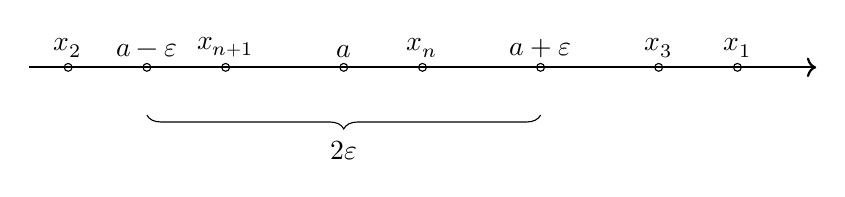
\begin{tikzpicture}
\draw[thick,->] (0,0) -- (10,0);
\draw (0.5,0) node[circle,draw,scale=0.3]{} node[above] {$x_2$};
\draw [decorate,decoration={brace,amplitude=5pt,mirror,raise=4ex}]
  (1.5,0) node[circle,draw,scale=0.3]{} node[above]{$a-\varepsilon$} -- (6.5,0) node[midway,yshift=-3em]{$2 \varepsilon$} node[circle,draw,scale=0.3]{} node[above]{$a+\varepsilon$};
%\draw [Parenthesis-Parenthesis,] (2,0) node[above] {$a-\varepsilon$} -- (7,0) node[above] {$a+\varepsilon$};
\draw (2.5,0) node[circle,draw,scale=0.3]{} node[above] {$x_{n+1}$};
\draw (4,0) node[circle,draw,scale=0.3]{} node[above] {$a$};
\draw (5,0) node[circle,draw,scale=0.3]{} node[above] {$x_n$};
%\draw (7,0) node[circle,draw,scale=0.3]{} node[above] {$a+\varepsilon$};
\draw (8,0) node[circle,draw,scale=0.3]{} node[above] {$x_3$};
\draw (9,0) node[circle,draw,scale=0.3]{} node[above] {$x_1$};
\end{tikzpicture}
\end{center}

以$a$点为中心的线段不论取的多小(其长度为$2\varepsilon$),一切$x_n$点从某点起,必全部落在这线段之内,这样在线段之外一定只有有限长度个点了,表示极限的点$a$表示整序变量的数值的点的凝聚中心.
\end{document}
